\documentclass[11pt,aspectratio=169]{beamer}
% =============================================================================
%  Shared Beamer preamble — Machine Learning I & II, PEU-CD 2026 (ENEI / INEI)
%
%  Inherited from the ML_Foundations deck (Alexander Quispe), with three changes:
%    * `minted` removed — it shells out to Pygments and does not build under
%      tectonic; every code block in the course uses `listings`.
%    * unused packages (lipsum, blindtext, multimedia, videoframe) dropped.
%    * `bbm` dropped — its fonts are PK-only and tectonic cannot render them;
%      the indicator uses \mathbf{1} instead.
%    * a math-macro block added so all twelve lectures share one notation.
%
%  Each lecture is a standalone document:
%      \documentclass[11pt,aspectratio=169]{beamer}
%      % =============================================================================
%  Shared Beamer preamble — Machine Learning I & II, PEU-CD 2026 (ENEI / INEI)
%
%  Inherited from the ML_Foundations deck (Alexander Quispe), with three changes:
%    * `minted` removed — it shells out to Pygments and does not build under
%      tectonic; every code block in the course uses `listings`.
%    * unused packages (lipsum, blindtext, multimedia, videoframe) dropped.
%    * `bbm` dropped — its fonts are PK-only and tectonic cannot render them;
%      the indicator uses \mathbf{1} instead.
%    * a math-macro block added so all twelve lectures share one notation.
%
%  Each lecture is a standalone document:
%      \documentclass[11pt,aspectratio=169]{beamer}
%      % =============================================================================
%  Shared Beamer preamble — Machine Learning I & II, PEU-CD 2026 (ENEI / INEI)
%
%  Inherited from the ML_Foundations deck (Alexander Quispe), with three changes:
%    * `minted` removed — it shells out to Pygments and does not build under
%      tectonic; every code block in the course uses `listings`.
%    * unused packages (lipsum, blindtext, multimedia, videoframe) dropped.
%    * `bbm` dropped — its fonts are PK-only and tectonic cannot render them;
%      the indicator uses \mathbf{1} instead.
%    * a math-macro block added so all twelve lectures share one notation.
%
%  Each lecture is a standalone document:
%      \documentclass[11pt,aspectratio=169]{beamer}
%      \input{../../../style/preamble}
% =============================================================================

% ---------- fonts ----------
\usepackage{helvet}
\usepackage[default]{lato}
\usepackage{tgbonum}
\usepackage{mathpazo}
\usepackage[utf8]{inputenc}

% ---------- math ----------
\usepackage{amsmath,amssymb}
\usepackage{mathtools}

% ---------- graphics, tables, layout ----------
\usepackage{graphicx}
\usepackage{tikz}
\usetikzlibrary{positioning,calc,arrows,arrows.meta,decorations.markings,shapes.misc,matrix,shapes,fit}
\usepackage{array}
\usepackage{booktabs}
\usepackage{multirow}
\usepackage{dcolumn}
\usepackage{subcaption}
\usepackage{caption}
\usepackage{changepage}
\usepackage{xspace}
\usepackage{tcolorbox}
\tcbuselibrary{skins,breakable}
\usepackage[ruled,vlined]{algorithm2e}
\usepackage{listings}
\usepackage{appendixnumberbeamer}
\usepackage{hyperref}

\newcolumntype{d}[0]{D{.}{.}{5}}
\setbeamertemplate{caption}[numbered]

% ---------- palette (Okabe–Ito, colour-blind safe) ----------
\definecolor{blue}{RGB}{0,114,178}
\definecolor{red}{RGB}{213,94,0}
\definecolor{yellow}{RGB}{240,228,66}
\definecolor{green}{RGB}{0,158,115}
\definecolor{MyBackground}{RGB}{255,253,218}

\hypersetup{colorlinks=true, linkbordercolor={white}, linkcolor={blue}, urlcolor={blue}}

% ---------- beamer look ----------
\setbeamercolor{frametitle}{fg=blue}
\setbeamercolor{title}{fg=black}
\setbeamertemplate{footline}[frame number]
\setbeamertemplate{navigation symbols}{}
\setbeamertemplate{itemize items}{-}
\setbeamercolor{itemize item}{fg=blue}
\setbeamercolor{itemize subitem}{fg=blue}
\setbeamercolor{enumerate item}{fg=blue}
\setbeamercolor{enumerate subitem}{fg=blue}
\setbeamercolor{button}{bg=MyBackground,fg=blue}
\setbeamercolor{section in toc}{fg=blue}
\setbeamercolor{subsection in toc}{fg=red}
\setbeamersize{text margin left=1em,text margin right=1em}
\setbeamercolor{block title}{fg=white,bg=blue}
\setbeamercolor{block body}{bg=blue!5}
\setbeamercolor{block title alerted}{fg=white,bg=red}
\setbeamercolor{block body alerted}{bg=red!5}
\setbeamercolor{block title example}{fg=white,bg=green}
\setbeamercolor{block body example}{bg=green!5}
\setbeamertemplate{blocks}[rounded][shadow=false]

\newenvironment{wideitemize}{\itemize\addtolength{\itemsep}{10pt}}{\enditemize}

\newenvironment{transitionframe}{
  \setbeamercolor{background canvas}{bg=yellow}
  \begin{frame}}{
  \end{frame}
}

% Section divider: a plain frame with a large blue title.
\newcommand{\sectionframe}[1]{%
  \section{#1}%
  \begin{frame}[plain]\vfill\begin{center}{\Huge\textcolor{blue}{#1}}\end{center}\vfill\end{frame}}

% ---------- proof / derivation environments ----------
% derivation: a boxed, step-by-step algebraic argument. Title is the claim.
\newtcolorbox{derivation}[1]{enhanced, colback=blue!3, colframe=blue, fonttitle=\bfseries,
  title={#1}, boxrule=0.6pt, left=4pt, right=4pt, top=3pt, bottom=3pt, arc=2pt}
% claim: a result to be proved (theorem / lemma / proposition).
\newtcolorbox{claim}[1]{enhanced, colback=white, colframe=black, fonttitle=\bfseries,
  title={#1}, boxrule=0.6pt, left=4pt, right=4pt, top=3pt, bottom=3pt, arc=2pt}
% keypoint: the one line to remember from a slide.
\newtcolorbox{keypoint}{enhanced, colback=green!6, colframe=green, boxrule=0.6pt,
  left=4pt, right=4pt, top=3pt, bottom=3pt, arc=2pt}
% caution: a common mistake or a subtlety.
\newtcolorbox{caution}{enhanced, colback=red!5, colframe=red, boxrule=0.6pt,
  left=4pt, right=4pt, top=3pt, bottom=3pt, arc=2pt}

% ---------- code ----------
\lstset{
  basicstyle=\ttfamily\scriptsize, keywordstyle=\color{blue}\bfseries,
  commentstyle=\color{green}, stringstyle=\color{red},
  showstringspaces=false, breaklines=true, frame=single, rulecolor=\color{black!30},
  numbers=none, xleftmargin=4pt, framexleftmargin=4pt, language=Python
}

\input{../../../style/macros}

% ---------- course-wide title metadata ----------
\newcommand{\courseinstitution}{ENEI -- INEI \,\textperiodcentered\, PEU-CD 2026}
\newcommand{\courseauthor}{Alexander Quispe}
\institute{\courseinstitution}
\author{\courseauthor}

% =============================================================================

% ---------- fonts ----------
\usepackage{helvet}
\usepackage[default]{lato}
\usepackage{tgbonum}
\usepackage{mathpazo}
\usepackage[utf8]{inputenc}

% ---------- math ----------
\usepackage{amsmath,amssymb}
\usepackage{mathtools}

% ---------- graphics, tables, layout ----------
\usepackage{graphicx}
\usepackage{tikz}
\usetikzlibrary{positioning,calc,arrows,arrows.meta,decorations.markings,shapes.misc,matrix,shapes,fit}
\usepackage{array}
\usepackage{booktabs}
\usepackage{multirow}
\usepackage{dcolumn}
\usepackage{subcaption}
\usepackage{caption}
\usepackage{changepage}
\usepackage{xspace}
\usepackage{tcolorbox}
\tcbuselibrary{skins,breakable}
\usepackage[ruled,vlined]{algorithm2e}
\usepackage{listings}
\usepackage{appendixnumberbeamer}
\usepackage{hyperref}

\newcolumntype{d}[0]{D{.}{.}{5}}
\setbeamertemplate{caption}[numbered]

% ---------- palette (Okabe–Ito, colour-blind safe) ----------
\definecolor{blue}{RGB}{0,114,178}
\definecolor{red}{RGB}{213,94,0}
\definecolor{yellow}{RGB}{240,228,66}
\definecolor{green}{RGB}{0,158,115}
\definecolor{MyBackground}{RGB}{255,253,218}

\hypersetup{colorlinks=true, linkbordercolor={white}, linkcolor={blue}, urlcolor={blue}}

% ---------- beamer look ----------
\setbeamercolor{frametitle}{fg=blue}
\setbeamercolor{title}{fg=black}
\setbeamertemplate{footline}[frame number]
\setbeamertemplate{navigation symbols}{}
\setbeamertemplate{itemize items}{-}
\setbeamercolor{itemize item}{fg=blue}
\setbeamercolor{itemize subitem}{fg=blue}
\setbeamercolor{enumerate item}{fg=blue}
\setbeamercolor{enumerate subitem}{fg=blue}
\setbeamercolor{button}{bg=MyBackground,fg=blue}
\setbeamercolor{section in toc}{fg=blue}
\setbeamercolor{subsection in toc}{fg=red}
\setbeamersize{text margin left=1em,text margin right=1em}
\setbeamercolor{block title}{fg=white,bg=blue}
\setbeamercolor{block body}{bg=blue!5}
\setbeamercolor{block title alerted}{fg=white,bg=red}
\setbeamercolor{block body alerted}{bg=red!5}
\setbeamercolor{block title example}{fg=white,bg=green}
\setbeamercolor{block body example}{bg=green!5}
\setbeamertemplate{blocks}[rounded][shadow=false]

\newenvironment{wideitemize}{\itemize\addtolength{\itemsep}{10pt}}{\enditemize}

\newenvironment{transitionframe}{
  \setbeamercolor{background canvas}{bg=yellow}
  \begin{frame}}{
  \end{frame}
}

% Section divider: a plain frame with a large blue title.
\newcommand{\sectionframe}[1]{%
  \section{#1}%
  \begin{frame}[plain]\vfill\begin{center}{\Huge\textcolor{blue}{#1}}\end{center}\vfill\end{frame}}

% ---------- proof / derivation environments ----------
% derivation: a boxed, step-by-step algebraic argument. Title is the claim.
\newtcolorbox{derivation}[1]{enhanced, colback=blue!3, colframe=blue, fonttitle=\bfseries,
  title={#1}, boxrule=0.6pt, left=4pt, right=4pt, top=3pt, bottom=3pt, arc=2pt}
% claim: a result to be proved (theorem / lemma / proposition).
\newtcolorbox{claim}[1]{enhanced, colback=white, colframe=black, fonttitle=\bfseries,
  title={#1}, boxrule=0.6pt, left=4pt, right=4pt, top=3pt, bottom=3pt, arc=2pt}
% keypoint: the one line to remember from a slide.
\newtcolorbox{keypoint}{enhanced, colback=green!6, colframe=green, boxrule=0.6pt,
  left=4pt, right=4pt, top=3pt, bottom=3pt, arc=2pt}
% caution: a common mistake or a subtlety.
\newtcolorbox{caution}{enhanced, colback=red!5, colframe=red, boxrule=0.6pt,
  left=4pt, right=4pt, top=3pt, bottom=3pt, arc=2pt}

% ---------- code ----------
\lstset{
  basicstyle=\ttfamily\scriptsize, keywordstyle=\color{blue}\bfseries,
  commentstyle=\color{green}, stringstyle=\color{red},
  showstringspaces=false, breaklines=true, frame=single, rulecolor=\color{black!30},
  numbers=none, xleftmargin=4pt, framexleftmargin=4pt, language=Python
}

% =============================================================================
%  Notation — one convention for all lectures
%
%  scalars      x, y, w           plain italic
%  vectors      \vx \vy \vw       bold lower-case
%  matrices     \vX \vW \vSigma   bold upper-case
%  parameters   \vbeta \vtheta    bold Greek
%  transpose    \vX\T             \top
% =============================================================================
\newcommand{\R}{\mathbb{R}}
\newcommand{\E}{\mathbb{E}}
\newcommand{\Prob}{\mathbb{P}}
\DeclareMathOperator{\Var}{Var}
\DeclareMathOperator{\Cov}{Cov}
\DeclareMathOperator{\tr}{tr}
\DeclareMathOperator{\diag}{diag}
\DeclareMathOperator{\rank}{rank}
\DeclareMathOperator{\sign}{sign}
\DeclareMathOperator{\col}{col}
\DeclareMathOperator{\RSS}{RSS}
\DeclareMathOperator*{\argmin}{arg\,min}
\DeclareMathOperator*{\argmax}{arg\,max}
\newcommand{\norm}[1]{\left\lVert #1 \right\rVert}
\newcommand{\abs}[1]{\left\lvert #1 \right\rvert}
\newcommand{\inner}[2]{\left\langle #1,\, #2 \right\rangle}
\newcommand{\ind}[1]{\mathbf{1}\!\left\{#1\right\}}
\newcommand{\T}{^{\top}}
\newcommand{\inv}{^{-1}}
\newcommand{\half}{\tfrac{1}{2}}
\newcommand{\eps}{\varepsilon}
\newcommand{\Dset}{\mathcal{D}}
\newcommand{\Hset}{\mathcal{H}}
\newcommand{\Lcal}{\mathcal{L}}
\newcommand{\Ncal}{\mathcal{N}}

% bold vectors
\newcommand{\vx}{\mathbf{x}}   \newcommand{\vy}{\mathbf{y}}   \newcommand{\vz}{\mathbf{z}}
\newcommand{\vw}{\mathbf{w}}   \newcommand{\vu}{\mathbf{u}}   \newcommand{\vv}{\mathbf{v}}
\newcommand{\vb}{\mathbf{b}}   \newcommand{\vh}{\mathbf{h}}   \newcommand{\vr}{\mathbf{r}}
\newcommand{\vc}{\mathbf{c}}   \newcommand{\vf}{\mathbf{f}}   \newcommand{\vg}{\mathbf{g}}
\newcommand{\vp}{\mathbf{p}}   \newcommand{\vq}{\mathbf{q}}   \newcommand{\vs}{\mathbf{s}}
\newcommand{\va}{\mathbf{a}}   \newcommand{\vd}{\mathbf{d}}   \newcommand{\vt}{\mathbf{t}}
\newcommand{\vk}{\mathbf{k}}   \newcommand{\vm}{\mathbf{m}}   \newcommand{\vn}{\mathbf{n}}
\newcommand{\vzero}{\mathbf{0}} \newcommand{\vone}{\mathbf{1}}
% bold matrices
\newcommand{\vX}{\mathbf{X}}   \newcommand{\vY}{\mathbf{Y}}   \newcommand{\vZ}{\mathbf{Z}}
\newcommand{\vW}{\mathbf{W}}   \newcommand{\vH}{\mathbf{H}}   \newcommand{\vI}{\mathbf{I}}
\newcommand{\vA}{\mathbf{A}}   \newcommand{\vB}{\mathbf{B}}   \newcommand{\vC}{\mathbf{C}}
\newcommand{\vD}{\mathbf{D}}   \newcommand{\vP}{\mathbf{P}}   \newcommand{\vQ}{\mathbf{Q}}
\newcommand{\vU}{\mathbf{U}}   \newcommand{\vV}{\mathbf{V}}   \newcommand{\vS}{\mathbf{S}}
\newcommand{\vM}{\mathbf{M}}   \newcommand{\vK}{\mathbf{K}}   \newcommand{\vG}{\mathbf{G}}
% bold Greek
\newcommand{\vbeta}{\boldsymbol{\beta}}     \newcommand{\valpha}{\boldsymbol{\alpha}}
\newcommand{\vtheta}{\boldsymbol{\theta}}   \newcommand{\vmu}{\boldsymbol{\mu}}
\newcommand{\vSigma}{\boldsymbol{\Sigma}}   \newcommand{\vLambda}{\boldsymbol{\Lambda}}
\newcommand{\veps}{\boldsymbol{\varepsilon}} \newcommand{\vphi}{\boldsymbol{\phi}}
\newcommand{\vgamma}{\boldsymbol{\gamma}}   \newcommand{\vlambda}{\boldsymbol{\lambda}}
\newcommand{\vdelta}{\boldsymbol{\delta}}   \newcommand{\vnu}{\boldsymbol{\nu}}
\newcommand{\vxi}{\boldsymbol{\xi}}         \newcommand{\vpi}{\boldsymbol{\pi}}
\newcommand{\vomega}{\boldsymbol{\omega}}



% ---------- course-wide title metadata ----------
\newcommand{\courseinstitution}{ENEI -- INEI \,\textperiodcentered\, PEU-CD 2026}
\newcommand{\courseauthor}{Alexander Quispe}
\institute{\courseinstitution}
\author{\courseauthor}

% =============================================================================

% ---------- fonts ----------
\usepackage{helvet}
\usepackage[default]{lato}
\usepackage{tgbonum}
\usepackage{mathpazo}
\usepackage[utf8]{inputenc}

% ---------- math ----------
\usepackage{amsmath,amssymb}
\usepackage{mathtools}

% ---------- graphics, tables, layout ----------
\usepackage{graphicx}
\usepackage{tikz}
\usetikzlibrary{positioning,calc,arrows,arrows.meta,decorations.markings,shapes.misc,matrix,shapes,fit}
\usepackage{array}
\usepackage{booktabs}
\usepackage{multirow}
\usepackage{dcolumn}
\usepackage{subcaption}
\usepackage{caption}
\usepackage{changepage}
\usepackage{xspace}
\usepackage{tcolorbox}
\tcbuselibrary{skins,breakable}
\usepackage[ruled,vlined]{algorithm2e}
\usepackage{listings}
\usepackage{appendixnumberbeamer}
\usepackage{hyperref}

\newcolumntype{d}[0]{D{.}{.}{5}}
\setbeamertemplate{caption}[numbered]

% ---------- palette (Okabe–Ito, colour-blind safe) ----------
\definecolor{blue}{RGB}{0,114,178}
\definecolor{red}{RGB}{213,94,0}
\definecolor{yellow}{RGB}{240,228,66}
\definecolor{green}{RGB}{0,158,115}
\definecolor{MyBackground}{RGB}{255,253,218}

\hypersetup{colorlinks=true, linkbordercolor={white}, linkcolor={blue}, urlcolor={blue}}

% ---------- beamer look ----------
\setbeamercolor{frametitle}{fg=blue}
\setbeamercolor{title}{fg=black}
\setbeamertemplate{footline}[frame number]
\setbeamertemplate{navigation symbols}{}
\setbeamertemplate{itemize items}{-}
\setbeamercolor{itemize item}{fg=blue}
\setbeamercolor{itemize subitem}{fg=blue}
\setbeamercolor{enumerate item}{fg=blue}
\setbeamercolor{enumerate subitem}{fg=blue}
\setbeamercolor{button}{bg=MyBackground,fg=blue}
\setbeamercolor{section in toc}{fg=blue}
\setbeamercolor{subsection in toc}{fg=red}
\setbeamersize{text margin left=1em,text margin right=1em}
\setbeamercolor{block title}{fg=white,bg=blue}
\setbeamercolor{block body}{bg=blue!5}
\setbeamercolor{block title alerted}{fg=white,bg=red}
\setbeamercolor{block body alerted}{bg=red!5}
\setbeamercolor{block title example}{fg=white,bg=green}
\setbeamercolor{block body example}{bg=green!5}
\setbeamertemplate{blocks}[rounded][shadow=false]

\newenvironment{wideitemize}{\itemize\addtolength{\itemsep}{10pt}}{\enditemize}

\newenvironment{transitionframe}{
  \setbeamercolor{background canvas}{bg=yellow}
  \begin{frame}}{
  \end{frame}
}

% Section divider: a plain frame with a large blue title.
\newcommand{\sectionframe}[1]{%
  \section{#1}%
  \begin{frame}[plain]\vfill\begin{center}{\Huge\textcolor{blue}{#1}}\end{center}\vfill\end{frame}}

% ---------- proof / derivation environments ----------
% derivation: a boxed, step-by-step algebraic argument. Title is the claim.
\newtcolorbox{derivation}[1]{enhanced, colback=blue!3, colframe=blue, fonttitle=\bfseries,
  title={#1}, boxrule=0.6pt, left=4pt, right=4pt, top=3pt, bottom=3pt, arc=2pt}
% claim: a result to be proved (theorem / lemma / proposition).
\newtcolorbox{claim}[1]{enhanced, colback=white, colframe=black, fonttitle=\bfseries,
  title={#1}, boxrule=0.6pt, left=4pt, right=4pt, top=3pt, bottom=3pt, arc=2pt}
% keypoint: the one line to remember from a slide.
\newtcolorbox{keypoint}{enhanced, colback=green!6, colframe=green, boxrule=0.6pt,
  left=4pt, right=4pt, top=3pt, bottom=3pt, arc=2pt}
% caution: a common mistake or a subtlety.
\newtcolorbox{caution}{enhanced, colback=red!5, colframe=red, boxrule=0.6pt,
  left=4pt, right=4pt, top=3pt, bottom=3pt, arc=2pt}

% ---------- code ----------
\lstset{
  basicstyle=\ttfamily\scriptsize, keywordstyle=\color{blue}\bfseries,
  commentstyle=\color{green}, stringstyle=\color{red},
  showstringspaces=false, breaklines=true, frame=single, rulecolor=\color{black!30},
  numbers=none, xleftmargin=4pt, framexleftmargin=4pt, language=Python
}

% =============================================================================
%  Notation — one convention for all lectures
%
%  scalars      x, y, w           plain italic
%  vectors      \vx \vy \vw       bold lower-case
%  matrices     \vX \vW \vSigma   bold upper-case
%  parameters   \vbeta \vtheta    bold Greek
%  transpose    \vX\T             \top
% =============================================================================
\newcommand{\R}{\mathbb{R}}
\newcommand{\E}{\mathbb{E}}
\newcommand{\Prob}{\mathbb{P}}
\DeclareMathOperator{\Var}{Var}
\DeclareMathOperator{\Cov}{Cov}
\DeclareMathOperator{\tr}{tr}
\DeclareMathOperator{\diag}{diag}
\DeclareMathOperator{\rank}{rank}
\DeclareMathOperator{\sign}{sign}
\DeclareMathOperator{\col}{col}
\DeclareMathOperator{\RSS}{RSS}
\DeclareMathOperator*{\argmin}{arg\,min}
\DeclareMathOperator*{\argmax}{arg\,max}
\newcommand{\norm}[1]{\left\lVert #1 \right\rVert}
\newcommand{\abs}[1]{\left\lvert #1 \right\rvert}
\newcommand{\inner}[2]{\left\langle #1,\, #2 \right\rangle}
\newcommand{\ind}[1]{\mathbf{1}\!\left\{#1\right\}}
\newcommand{\T}{^{\top}}
\newcommand{\inv}{^{-1}}
\newcommand{\half}{\tfrac{1}{2}}
\newcommand{\eps}{\varepsilon}
\newcommand{\Dset}{\mathcal{D}}
\newcommand{\Hset}{\mathcal{H}}
\newcommand{\Lcal}{\mathcal{L}}
\newcommand{\Ncal}{\mathcal{N}}

% bold vectors
\newcommand{\vx}{\mathbf{x}}   \newcommand{\vy}{\mathbf{y}}   \newcommand{\vz}{\mathbf{z}}
\newcommand{\vw}{\mathbf{w}}   \newcommand{\vu}{\mathbf{u}}   \newcommand{\vv}{\mathbf{v}}
\newcommand{\vb}{\mathbf{b}}   \newcommand{\vh}{\mathbf{h}}   \newcommand{\vr}{\mathbf{r}}
\newcommand{\vc}{\mathbf{c}}   \newcommand{\vf}{\mathbf{f}}   \newcommand{\vg}{\mathbf{g}}
\newcommand{\vp}{\mathbf{p}}   \newcommand{\vq}{\mathbf{q}}   \newcommand{\vs}{\mathbf{s}}
\newcommand{\va}{\mathbf{a}}   \newcommand{\vd}{\mathbf{d}}   \newcommand{\vt}{\mathbf{t}}
\newcommand{\vk}{\mathbf{k}}   \newcommand{\vm}{\mathbf{m}}   \newcommand{\vn}{\mathbf{n}}
\newcommand{\vzero}{\mathbf{0}} \newcommand{\vone}{\mathbf{1}}
% bold matrices
\newcommand{\vX}{\mathbf{X}}   \newcommand{\vY}{\mathbf{Y}}   \newcommand{\vZ}{\mathbf{Z}}
\newcommand{\vW}{\mathbf{W}}   \newcommand{\vH}{\mathbf{H}}   \newcommand{\vI}{\mathbf{I}}
\newcommand{\vA}{\mathbf{A}}   \newcommand{\vB}{\mathbf{B}}   \newcommand{\vC}{\mathbf{C}}
\newcommand{\vD}{\mathbf{D}}   \newcommand{\vP}{\mathbf{P}}   \newcommand{\vQ}{\mathbf{Q}}
\newcommand{\vU}{\mathbf{U}}   \newcommand{\vV}{\mathbf{V}}   \newcommand{\vS}{\mathbf{S}}
\newcommand{\vM}{\mathbf{M}}   \newcommand{\vK}{\mathbf{K}}   \newcommand{\vG}{\mathbf{G}}
% bold Greek
\newcommand{\vbeta}{\boldsymbol{\beta}}     \newcommand{\valpha}{\boldsymbol{\alpha}}
\newcommand{\vtheta}{\boldsymbol{\theta}}   \newcommand{\vmu}{\boldsymbol{\mu}}
\newcommand{\vSigma}{\boldsymbol{\Sigma}}   \newcommand{\vLambda}{\boldsymbol{\Lambda}}
\newcommand{\veps}{\boldsymbol{\varepsilon}} \newcommand{\vphi}{\boldsymbol{\phi}}
\newcommand{\vgamma}{\boldsymbol{\gamma}}   \newcommand{\vlambda}{\boldsymbol{\lambda}}
\newcommand{\vdelta}{\boldsymbol{\delta}}   \newcommand{\vnu}{\boldsymbol{\nu}}
\newcommand{\vxi}{\boldsymbol{\xi}}         \newcommand{\vpi}{\boldsymbol{\pi}}
\newcommand{\vomega}{\boldsymbol{\omega}}



% ---------- course-wide title metadata ----------
\newcommand{\courseinstitution}{ENEI -- INEI \,\textperiodcentered\, PEU-CD 2026}
\newcommand{\courseauthor}{Alexander Quispe}
\institute{\courseinstitution}
\author{\courseauthor}

\graphicspath{{figures/}}

\title{\textcolor{blue}{Lecture 3 \\ Regularization and Evaluation}}
\subtitle{Machine Learning I}
\date{September 14, 2026}

\begin{document}

\begin{frame}[plain]
\maketitle
\end{frame}

\begin{frame}{Outline}
\tableofcontents
\end{frame}

\begin{frame}{Two Loose Ends From Lectures 1--2}
\begin{enumerate}
  \item Least squares has variance $\sigma^2\,\tfrac{p+1}{N}$, growing with every feature. When $p$ approaches
        $N$ --- or when columns are nearly collinear --- $(\vX\T\vX)\inv$ explodes and so does $\hat\vbeta$.
  \item Logistic regression on separable data has no MLE: $\norm{\hat\vbeta}\to\infty$.
\end{enumerate}
\vspace{4pt}
Both are the same disease: nothing in the objective stops $\vbeta$ from being large.
\begin{block}{The cure}
Add a penalty on the size of $\vbeta$ to the empirical risk:
\[
\hat\vbeta_\lambda=\argmin_{\vbeta}\ \hat R(\vbeta)+\lambda\,\Omega(\vbeta),\qquad\lambda\ge0 .
\]
\end{block}
Today: $\Omega=\norm\vbeta_2^2$ (ridge), $\Omega=\norm\vbeta_1$ (lasso), what each does to the solution and why,
how to pick $\lambda$, and --- second half --- how to score a classifier at all.
\end{frame}

% =============================================================================
\sectionframe{Ridge Regression}
% =============================================================================

\begin{frame}{The Objective and Its Closed Form}
\[
J_\lambda(\vbeta)=\norm{\vy-\vX\vbeta}^2+\lambda\norm{\vbeta}^2
=(\vy-\vX\vbeta)\T(\vy-\vX\vbeta)+\lambda\vbeta\T\vbeta .
\]
\begin{derivation}{Gradient, then normal equations}
Reuse Lecture 1 for the first term; the second is a quadratic form with $\vA=\lambda\vI$:
\[
\nabla_{\vbeta}J_\lambda=-2\vX\T(\vy-\vX\vbeta)+2\lambda\vbeta=2\bigl[(\vX\T\vX+\lambda\vI)\vbeta-\vX\T\vy\bigr].
\]
Setting it to zero,
\[
\boxed{\ \hat\vbeta_\lambda=(\vX\T\vX+\lambda\vI)\inv\vX\T\vy\ }
\]
\end{derivation}
\begin{itemize}
  \item $\lambda=0$ recovers least squares. $\lambda\to\infty$ drives $\hat\vbeta_\lambda\to\vzero$.
  \item The Hessian is $2(\vX\T\vX+\lambda\vI)$; next slide shows it is positive definite for every $\lambda>0$,
        so the solution is unique --- \emph{regardless of the rank of }$\vX$.
\end{itemize}
\end{frame}

\begin{frame}{Invertibility}
\begin{claim}{For $\lambda>0$, $\vX\T\vX+\lambda\vI$ is positive definite, hence invertible}
For any $\vv\neq\vzero$,
\[
\vv\T(\vX\T\vX+\lambda\vI)\vv=\norm{\vX\vv}^2+\lambda\norm{\vv}^2\ \ge\ \lambda\norm\vv^2\ >\ 0 .
\]
A symmetric matrix with all quadratic forms positive has all eigenvalues positive, so it is invertible. \qed
\end{claim}
\vspace{4pt}
\begin{itemize}
  \item Each eigenvalue of $\vX\T\vX$ is shifted up by $\lambda$: $\lambda_j(\vX\T\vX+\lambda\vI)=\lambda_j(\vX\T\vX)+\lambda$.
        Zero eigenvalues (collinearity, $p>N$) become $\lambda$.
  \item This is the origin of the name: the diagonal of $\vX\T\vX$ gets a ``ridge''.
\end{itemize}
\begin{keypoint}
Ridge always has a unique solution, including when $p>N$. That alone justifies it.
\end{keypoint}
\end{frame}

\begin{frame}{Ridge Is Biased}
\begin{derivation}{$\E[\hat\vbeta_\lambda]\neq\vbeta$}
Under $\vy=\vX\vbeta+\veps$, $\E[\veps]=\vzero$,
\[
\E[\hat\vbeta_\lambda]=(\vX\T\vX+\lambda\vI)\inv\vX\T\,\E[\vy]=(\vX\T\vX+\lambda\vI)\inv\vX\T\vX\,\vbeta
=\bigl(\vI+\lambda(\vX\T\vX)\inv\bigr)\inv\vbeta .
\]
\end{derivation}
\begin{derivation}{Variance}
\[
\Var(\hat\vbeta_\lambda)=\sigma^2(\vX\T\vX+\lambda\vI)\inv\vX\T\vX(\vX\T\vX+\lambda\vI)\inv
\ \preceq\ \sigma^2(\vX\T\vX)\inv=\Var(\hat\vbeta_{\text{OLS}}) .
\]
\end{derivation}
Bias in, variance out. Whether the trade is worth it depends on $\lambda$ --- and there always exists a
$\lambda>0$ for which the total mean squared error of $\hat\vbeta_\lambda$ is below that of OLS
(Hoerl \& Kennard, 1970). The proof is in the homework; the mechanism is on the next two slides.
\end{frame}

\begin{frame}{Ridge in the SVD Basis}\footnotesize
Write the thin SVD $\vX=\vU\vD\vV\T$: $\vU\in\R^{N\times p}$ orthonormal columns, $\vD=\diag(d_1,\dots,d_p)$,
$\vV\in\R^{p\times p}$ orthogonal. Then $\vX\T\vX=\vV\vD^2\vV\T$.
\begin{derivation}{The fitted values, direction by direction}
\begin{align*}
\hat\vy_\lambda=\vX\hat\vbeta_\lambda
&=\vU\vD\vV\T\bigl(\vV\vD^2\vV\T+\lambda\vV\vV\T\bigr)\inv\vV\vD\vU\T\vy
&&\text{($\vI=\vV\vV\T$)}\\
&=\vU\vD\vV\T\,\vV(\vD^2+\lambda\vI)\inv\vV\T\,\vV\vD\vU\T\vy
=\vU\vD(\vD^2+\lambda\vI)\inv\vD\,\vU\T\vy\\
&=\sum_{j=1}^p\vu_j\,\frac{d_j^2}{d_j^2+\lambda}\,\vu_j\T\vy .
\end{align*}
\end{derivation}
Compare least squares: $\hat\vy=\vU\vU\T\vy=\sum_j\vu_j\,\vu_j\T\vy$.
\begin{keypoint}
Ridge projects $\vy$ onto each principal direction $\vu_j$ of $\vX$, then \textbf{shrinks} the coordinate by
$\dfrac{d_j^2}{d_j^2+\lambda}\in(0,1)$. Directions with small $d_j$ --- low variance in the inputs, high
variance in $\hat\vbeta$ --- are shrunk the most. That is precisely where OLS variance lives.
\end{keypoint}
\end{frame}

\begin{frame}{Shrinkage Factors and Effective Degrees of Freedom}
\begin{center}
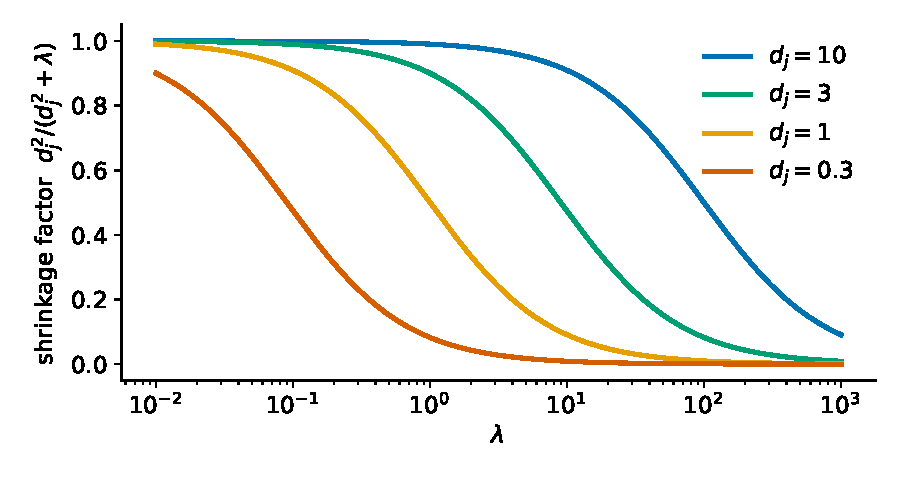
\includegraphics[height=0.45\textheight]{fig_ridge_shrinkage.pdf}
\end{center}
\vspace{-4pt}
The trace of the ridge hat matrix $\vH_\lambda=\vX(\vX\T\vX+\lambda\vI)\inv\vX\T$ generalizes Lecture 1's $\tr\vH=p$:
\[
\mathrm{df}(\lambda)=\tr\vH_\lambda=\sum_{j=1}^p\frac{d_j^2}{d_j^2+\lambda},\qquad
\mathrm{df}(0)=p,\quad\mathrm{df}(\infty)=0 .
\]
A fractional number of parameters. It is the right $x$-axis for a bias--variance plot.
\end{frame}

\begin{frame}{Two Practical Rules}
\begin{caution}
\textbf{Do not penalize the intercept.} Shrinking $\beta_0$ toward $0$ makes the fit depend on where the
origin of $y$ happens to be. Center $\vy$ and the columns of $\vX$ first; then $\hat\beta_0=\bar y$ and the
ridge problem is solved on the $p$ slopes only.
\end{caution}
\begin{caution}
\textbf{Standardize the features.} $\norm\vbeta^2$ treats all coordinates alike; a feature measured in
metres and the same feature in millimetres get coefficients differing by $10^3$ and penalties differing by
$10^6$. Divide each column by its standard deviation before fitting, and undo it afterwards.
\end{caution}
\vspace{4pt}
Both rules apply verbatim to the lasso.
\end{frame}

\begin{frame}{Ridge as a Bayesian Posterior Mode}\small
Take the Gaussian model of Lecture 1 and add a prior on $\vbeta$:
\[
\vy\mid\vbeta\sim\Ncal(\vX\vbeta,\sigma^2\vI),\qquad\vbeta\sim\Ncal(\vzero,\tau^2\vI).
\]
\begin{derivation}{Maximize the log posterior}
\begin{align*}
\log p(\vbeta\mid\vy)&=\log p(\vy\mid\vbeta)+\log p(\vbeta)+\text{const}\\
&=-\frac{1}{2\sigma^2}\norm{\vy-\vX\vbeta}^2-\frac{1}{2\tau^2}\norm\vbeta^2+\text{const}
=-\frac{1}{2\sigma^2}\Bigl[\norm{\vy-\vX\vbeta}^2+\frac{\sigma^2}{\tau^2}\norm\vbeta^2\Bigr]+\text{const}.
\end{align*}
Maximizing over $\vbeta$ is minimizing $J_\lambda$ with $\lambda=\sigma^2/\tau^2$.
\end{derivation}
\begin{itemize}
  \item A tight prior (small $\tau$) is a large $\lambda$. The penalty encodes a belief that coefficients are small.
  \item The same computation with a Laplace prior $p(\beta_j)\propto e^{-\abs{\beta_j}/b}$ gives the lasso, $\lambda=2\sigma^2/b$.
  \item This is the cleanest answer to ``where does the penalty come from''. It is also why the two are called
        $\ell_2$ and $\ell_1$ regularization: they are the log-densities of the two priors.
\end{itemize}
\end{frame}

% =============================================================================
\sectionframe{Penalties and Constraints}
% =============================================================================

\begin{frame}{Two Formulations}
\begin{columns}[T]
\begin{column}{0.48\textwidth}
\textbf{Penalized}
\[
\min_{\vbeta}\ L(\vbeta)+\lambda\,\Omega(\vbeta)
\]
One parameter $\lambda\ge0$.
\end{column}
\begin{column}{0.48\textwidth}
\textbf{Constrained}
\[
\min_{\vbeta}\ L(\vbeta)\quad\text{s.t.}\quad\Omega(\vbeta)\le t
\]
One parameter $t\ge0$.
\end{column}
\end{columns}
\vspace{10pt}
\begin{claim}{Equivalence}
For convex $L$ and $\Omega$: every solution of the penalized problem with parameter $\lambda$ solves the
constrained problem with $t=\Omega(\hat\vbeta_\lambda)$; and every solution of the constrained problem with
$t>0$ solves the penalized problem for some $\lambda\ge0$.
\end{claim}
The map $\lambda\leftrightarrow t$ is monotone decreasing but depends on the data --- one cannot convert
without solving. The constrained form is the one to \emph{draw}; the penalized form is the one to \emph{compute}.
\end{frame}

\begin{frame}{Equivalence: Both Directions}\small
\begin{derivation}{Penalized $\Rightarrow$ constrained (no convexity needed)}
Let $\hat\vbeta_\lambda$ minimize $L+\lambda\Omega$ and set $t=\Omega(\hat\vbeta_\lambda)$. For any $\vbeta$ with $\Omega(\vbeta)\le t$,
\[
L(\vbeta)\ \ge\ L(\hat\vbeta_\lambda)+\lambda\bigl[\Omega(\hat\vbeta_\lambda)-\Omega(\vbeta)\bigr]
\ =\ L(\hat\vbeta_\lambda)+\lambda\bigl[t-\Omega(\vbeta)\bigr]\ \ge\ L(\hat\vbeta_\lambda),
\]
the first inequality being the optimality of $\hat\vbeta_\lambda$ for the penalized objective. So $\hat\vbeta_\lambda$ is feasible and no feasible point beats it. \qed
\end{derivation}
\begin{derivation}{Constrained $\Rightarrow$ penalized (convexity used here)}
The constrained problem is convex with a strictly feasible point ($\vbeta=\vzero$, if $t>0$), so Slater's
condition holds and strong duality applies: there is a multiplier $\lambda^\star\ge0$ such that the
constrained minimizer $\hat\vbeta_t$ minimizes the Lagrangian $L(\vbeta)+\lambda^\star\bigl(\Omega(\vbeta)-t\bigr)$
over all $\vbeta$. The $-\lambda^\star t$ is a constant, so $\hat\vbeta_t$ minimizes $L+\lambda^\star\Omega$. \qed
\end{derivation}
\end{frame}

\begin{frame}{The Picture}
\begin{center}
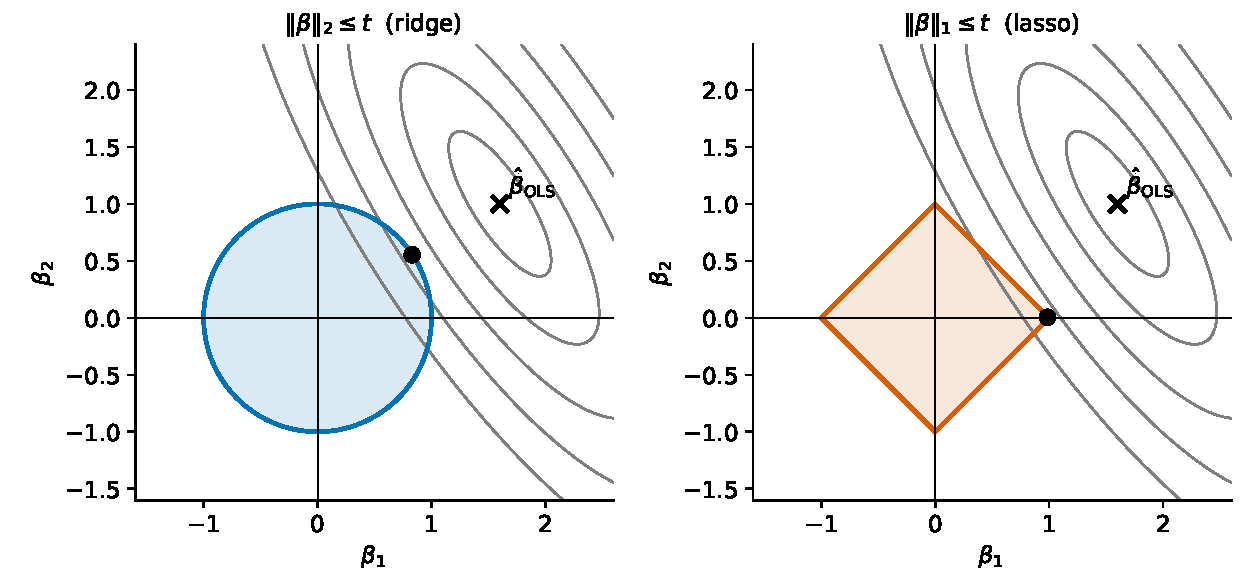
\includegraphics[height=0.6\textheight]{fig_l1_l2_geometry.pdf}
\end{center}
\vspace{-6pt}
Contours of $\norm{\vy-\vX\vbeta}^2$ (ellipses centred at $\hat\vbeta_{\text{OLS}}$) meeting the constraint set
$\Omega(\vbeta)\le t$. The $\ell_2$ ball is round: the first touch is almost never on an axis. The $\ell_1$
ball has corners on the axes: the first touch often is. The next section makes ``often'' precise.
\end{frame}

% =============================================================================
\sectionframe{The Lasso}
% =============================================================================

\begin{frame}{The Objective}
\[
J_\lambda(\vbeta)=\frac12\norm{\vy-\vX\vbeta}^2+\lambda\norm{\vbeta}_1,\qquad\norm\vbeta_1=\sum_{j=1}^p\abs{\beta_j}.
\]
(The $\tfrac12$ is a convention that removes a factor of 2 from every formula below.)
\begin{itemize}
  \item Convex: a convex quadratic plus a norm. Every local minimum is global.
  \item Not differentiable wherever some $\beta_j=0$. No closed form for general $\vX$.
  \item Solutions are typically \textbf{sparse}: many $\hat\beta_j$ exactly $0$. Ridge never does this.
\end{itemize}
\begin{block}{Subgradient of the absolute value}
\[
\partial\abs{\beta}=\begin{cases}\{+1\} & \beta>0\\ [-1,+1] & \beta=0\\ \{-1\} & \beta<0\end{cases}
\qquad\text{and }\vbeta^\star\text{ minimizes convex }J\iff\vzero\in\partial J(\vbeta^\star).
\]
\end{block}
\end{frame}

\begin{frame}{The Orthonormal Case: Soft Thresholding}\footnotesize
Suppose $\vX\T\vX=\vI$ (columns orthonormal). Write $\vb=\vX\T\vy$; note $\vb=\hat\vbeta_{\text{OLS}}$.
\begin{derivation}{The problem separates across coordinates}
\[
\frac12\norm{\vy-\vX\vbeta}^2=\frac12\norm\vy^2-\vb\T\vbeta+\frac12\vbeta\T\underbrace{\vX\T\vX}_{\vI}\vbeta
\ \Rightarrow\
J_\lambda(\vbeta)=\text{const}+\sum_{j=1}^p\Bigl[\tfrac12\beta_j^2-b_j\beta_j+\lambda\abs{\beta_j}\Bigr].
\]
\end{derivation}
\begin{derivation}{Minimize one coordinate: $\ \min_\beta\ \tfrac12\beta^2-b\beta+\lambda\abs\beta$}
Stationarity: $0\in\beta-b+\lambda\,\partial\abs\beta$, i.e.\ $\beta=b-\lambda s$ for some $s\in\partial\abs\beta$.
\begin{itemize}
  \item If $\beta>0$: $s=1$, $\beta=b-\lambda$; consistent iff $b>\lambda$.
  \item If $\beta<0$: $s=-1$, $\beta=b+\lambda$; consistent iff $b<-\lambda$.
  \item If $\beta=0$: need $0=b-\lambda s$ with $s\in[-1,1]$, i.e.\ $\abs b\le\lambda$.
\end{itemize}
The three cases partition $\R$. Hence
\[
\boxed{\ \hat\beta_j=S_\lambda(b_j)\equiv\sign(b_j)\,\bigl(\abs{b_j}-\lambda\bigr)_+\ }
\]
\end{derivation}
\end{frame}

\begin{frame}{Soft Thresholding vs.\ Ridge Shrinkage}
In the same orthonormal setting, ridge gives $\hat\beta_j=(\vI+\lambda\vI)\inv b_j=\dfrac{b_j}{1+\lambda}$.
\begin{center}
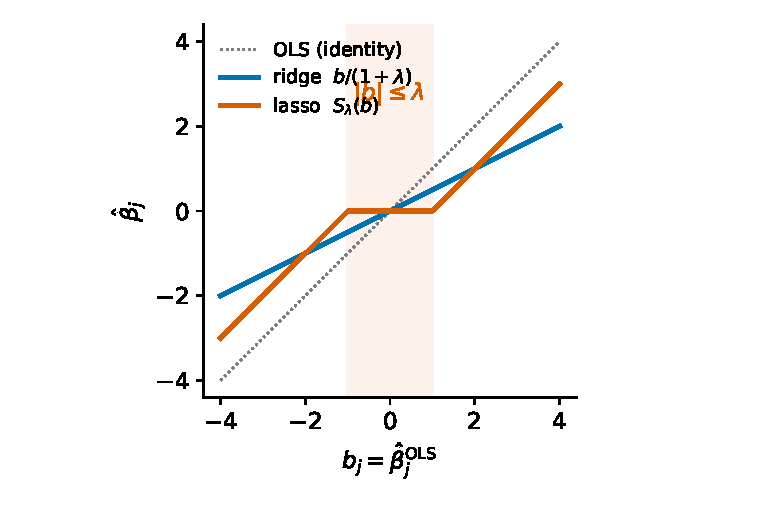
\includegraphics[height=0.45\textheight]{fig_soft_threshold.pdf}
\end{center}
\vspace{-4pt}
\begin{columns}[T]
\begin{column}{0.5\textwidth}
\textbf{Ridge:} multiply every coefficient by the same factor $<1$. Zero stays zero; nothing else becomes zero.
\end{column}
\begin{column}{0.5\textwidth}
\textbf{Lasso:} subtract $\lambda$ from every $\abs{b_j}$, floor at $0$. Everything with $\abs{b_j}\le\lambda$ is set to exactly zero.
\end{column}
\end{columns}
\end{frame}

\begin{frame}{Numerical Example}
Orthonormal design, $\vb=\hat\vbeta_{\text{OLS}}=(3,\ 0.5,\ -2)\T$, $\lambda=1$.
\begin{center}
\begin{tabular}{lccc}
\toprule
 & $b_1=3$ & $b_2=0.5$ & $b_3=-2$ \\
\midrule
Ridge $\ b_j/(1+\lambda)$ & $1.5$ & $0.25$ & $-1$ \\
Lasso $\ \sign(b_j)(\abs{b_j}-\lambda)_+$ & $2$ & $\mathbf{0}$ & $-1$ \\
\bottomrule
\end{tabular}
\end{center}
\vspace{4pt}
Ridge halves everything. Lasso removes the small coefficient and shifts the large ones by a constant ---
so the large ones are \emph{less} shrunk under lasso than under ridge here ($2$ vs $1.5$).
\begin{keypoint}
Lasso bias is roughly constant in $\abs{b_j}$; ridge bias is proportional to $\abs{b_j}$. Lasso hurts large
true coefficients less, and kills small ones outright.
\end{keypoint}
% verify: L3.soft_threshold_example
\end{frame}

\begin{frame}{General $\vX$: When Is $\hat\beta_j$ Exactly Zero?}\small
\begin{derivation}{KKT conditions for the lasso}
Stationarity, coordinate by coordinate, with $\vx^{(j)}$ the $j$-th column of $\vX$ and $\vr=\vy-\vX\hat\vbeta$:
\[
0\in-\vx^{(j)\top}\vr+\lambda\,\partial\abs{\hat\beta_j}
\qquad\Longleftrightarrow\qquad
\vx^{(j)\top}\vr=\lambda s_j,\quad s_j\in\partial\abs{\hat\beta_j}.
\]
\end{derivation}
Reading it:
\begin{itemize}
  \item If $\hat\beta_j\neq0$: $\vx^{(j)\top}\vr=\lambda\sign(\hat\beta_j)$. Every \emph{active} feature has correlation
        with the residual of magnitude exactly $\lambda$.
  \item If $\hat\beta_j=0$: $\abs{\vx^{(j)\top}\vr}\le\lambda$. An \emph{inactive} feature is one whose correlation
        with the residual does not reach $\lambda$.
\end{itemize}
\begin{keypoint}
A coefficient is zero iff its feature explains less than $\lambda$ worth of the residual. There is a whole
interval of $\lambda$ values for which this holds, so zeros are not a coincidence: they have positive probability.
\end{keypoint}
Corollary: $\hat\vbeta=\vzero$ iff $\abs{\vx^{(j)\top}\vy}\le\lambda$ for all $j$, i.e.\ iff $\lambda\ge\lambda_{\max}=\norm{\vX\T\vy}_\infty$.
The path starts there.
\end{frame}

\begin{frame}{Solving It: Coordinate Descent}\footnotesize
Fix all coordinates but $\beta_j$. Let $\vr_{(-j)}=\vy-\sum_{k\ne j}\vx^{(k)}\beta_k$ be the partial residual.
\begin{derivation}{One coordinate is a one-dimensional lasso}
\[
\frac12\norm{\vr_{(-j)}-\vx^{(j)}\beta_j}^2+\lambda\abs{\beta_j}
=\frac{\norm{\vx^{(j)}}^2}{2}\,\beta_j^2-\bigl(\vx^{(j)\top}\vr_{(-j)}\bigr)\beta_j+\lambda\abs{\beta_j}+\text{const}.
\]
Dividing by $\norm{\vx^{(j)}}^2$ puts it in the form of the orthonormal case, with $b=\vx^{(j)\top}\vr_{(-j)}/\norm{\vx^{(j)}}^2$
and threshold $\lambda/\norm{\vx^{(j)}}^2$:
\[
\boxed{\ \beta_j\leftarrow\frac{S_\lambda\bigl(\vx^{(j)\top}\vr_{(-j)}\bigr)}{\norm{\vx^{(j)}}^2}\ }
\]
\end{derivation}
\begin{itemize}
  \item Cycle $j=1,\dots,p$ until nothing changes. Each update is $O(N)$; a full sweep is $O(Np)$.
  \item Compute the whole path by starting at $\lambda_{\max}$ and decreasing $\lambda$ on a grid, warm-starting
        each solve from the previous one. This is what \texttt{glmnet} and scikit-learn do.
\end{itemize}
\end{frame}

\begin{frame}{The Lasso Path}
\begin{center}
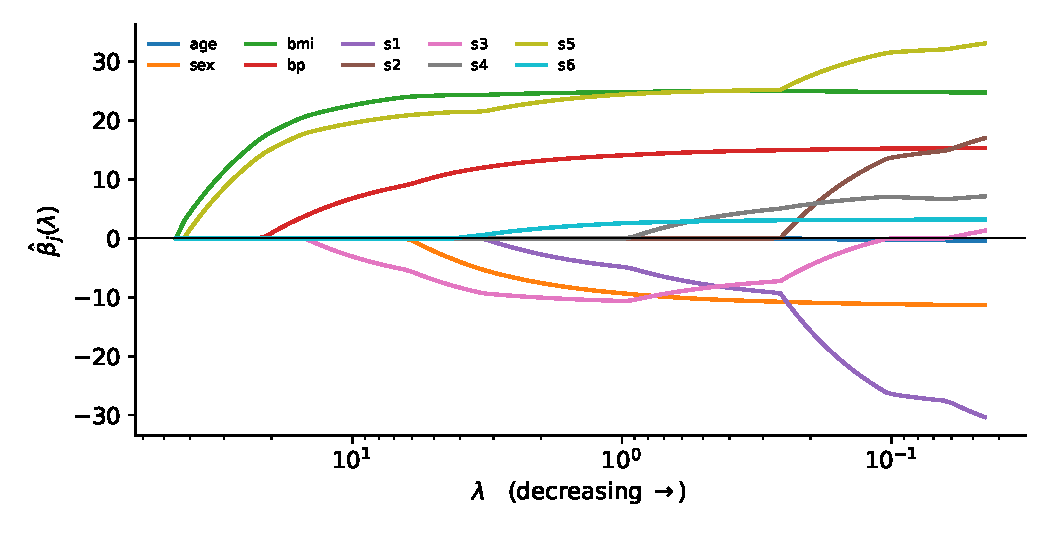
\includegraphics[height=0.62\textheight]{fig_lasso_path.pdf}
\end{center}
\vspace{-6pt}
Coefficients of the diabetes data as $\lambda$ decreases from $\lambda_{\max}$ (left) to $0$ (right).
Features enter one at a time, at the $\lambda$ where their correlation with the residual reaches $\lambda$.
The path is piecewise linear in $\lambda$ --- a fact that makes the whole thing computable exactly.
\end{frame}

\begin{frame}{Beyond Ridge and Lasso}
\begin{itemize}
  \item \textbf{Elastic net}: $\lambda_1\norm\vbeta_1+\lambda_2\norm\vbeta_2^2$. Keeps the sparsity of $\ell_1$, adds
        the stability of $\ell_2$ when features are correlated (lasso tends to pick one of a correlated group at random).
  \item \textbf{Regularized logistic regression}: replace $\tfrac12\norm{\vy-\vX\vbeta}^2$ by the log loss. The
        objective is strictly convex for any $\lambda>0$, so the separable-data problem of Lecture 2 disappears.
        Coordinate descent still works, via IRLS on each coordinate.
  \item \textbf{Early stopping} is regularization too: for gradient descent on least squares from $\vbeta=\vzero$,
        the iterate after $t$ steps shrinks direction $j$ by $1-(1-\eta d_j^2)^t$ --- the same shape as ridge's
        $d_j^2/(d_j^2+\lambda)$, with $t$ playing the role of $1/\lambda$.
\end{itemize}
\begin{keypoint}
Every method in this course has a knob that trades bias for variance. Ridge and lasso are the two whose
knob has a closed-form meaning.
\end{keypoint}
\end{frame}

% =============================================================================
\sectionframe{Choosing $\lambda$}
% =============================================================================

\begin{frame}{Training Error Is Optimistic --- By Exactly How Much}\footnotesize\vspace{-4pt}
For any \emph{linear smoother} $\hat\vy=\vH\vy$ (least squares, ridge, and others) under $\vy=\vf+\veps$, $\Var(\veps)=\sigma^2\vI$:
\begin{derivation}{Expected training error vs.\ expected test error at the same inputs}
Let $\vy'$ be a fresh copy of the responses at the same $\vX$. Then
\begin{align*}
\E\norm{\vy'-\hat\vy}^2-\E\norm{\vy-\hat\vy}^2
&=2\sum_{i=1}^N\Cov(y_i,\hat y_i)\\
&=2\sum_{i=1}^N\Cov\Bigl(y_i,\sum_kH_{ik}y_k\Bigr)=2\sigma^2\sum_iH_{ii}=2\sigma^2\tr\vH .
\end{align*}
Second line: expand both squares; $\vy'\perp\hat\vy$ kills one cross term, and $\E\norm{\vy'}^2=\E\norm\vy^2$.
\begin{align*}
\end{align*}
\end{derivation}
\[
\boxed{\ \E[\text{test error}]=\E[\text{training error}]+\frac{2\sigma^2}{N}\,\mathrm{df}\ }
\qquad\text{(per observation, }\mathrm{df}=\tr\vH\text{)}
\]
The optimism grows with the degrees of freedom. This is Mallows' $C_p$, and the reason $\mathrm{df}(\lambda)$ was
worth defining: it is the currency in which overfitting is paid.
\end{frame}

\begin{frame}{Cross-Validation}\small
When $\sigma^2$ and $\mathrm{df}$ are unknown --- most of the time --- estimate the test error directly.
\begin{algorithm}[H]
\SetAlgoLined
\KwIn{data $\Dset$, grid $\{\lambda_1,\dots,\lambda_m\}$, number of folds $K$}
Split $\Dset$ at random into $K$ folds $\Dset_1,\dots,\Dset_K$ of equal size\;
\For{$\lambda$ in the grid}{
  \For{$k=1,\dots,K$}{
    fit $\hat\vbeta_\lambda^{(-k)}$ on $\Dset\setminus\Dset_k$; \ $e_k(\lambda)\gets$ error of $\hat\vbeta_\lambda^{(-k)}$ on $\Dset_k$\;
  }
  $\mathrm{CV}(\lambda)\gets\frac1K\sum_ke_k(\lambda)$, \ $\mathrm{se}(\lambda)\gets\text{s.d.}\bigl(e_1,\dots,e_K\bigr)/\sqrt K$\;
}
\KwOut{$\hat\lambda=\argmin_\lambda\mathrm{CV}(\lambda)$, or the largest $\lambda$ with $\mathrm{CV}(\lambda)\le\min\mathrm{CV}+\mathrm{se}$}
\end{algorithm}
\begin{itemize}
  \item $K=5$ or $10$. Larger $K$: less bias (bigger training sets), more variance and cost.
  \item The \textbf{one-standard-error rule} picks the simplest model statistically indistinguishable from the best.
  \item Standardize \emph{inside} each fold. Standardizing once on all of $\Dset$ leaks the held-out fold's scale
        into training --- a small leak, but a leak.
\end{itemize}
\end{frame}

% =============================================================================
\sectionframe{Evaluating a Classifier}
% =============================================================================

\begin{frame}{Accuracy Is Not Enough}
A classifier outputs $\hat y\in\{0,1\}$; the truth is $y\in\{0,1\}$. Four outcomes:
\begin{center}
\begin{tabular}{l|cc}
 & $\hat y=1$ & $\hat y=0$ \\
\hline
$y=1$ & true positive (TP) & false negative (FN) \\
$y=0$ & false positive (FP) & true negative (TN) \\
\end{tabular}
\end{center}
\vspace{4pt}
\[
\text{Accuracy}=\frac{\text{TP}+\text{TN}}{N},\qquad
\text{Precision}=\frac{\text{TP}}{\text{TP}+\text{FP}},\qquad
\text{Recall}=\frac{\text{TP}}{\text{TP}+\text{FN}} .
\]
\begin{caution}
With $1\%$ positives, predicting ``0'' for everyone has $99\%$ accuracy, $0$ recall, and undefined precision.
Accuracy rewards agreeing with the majority. Precision and recall each measure one kind of mistake.
\end{caution}
The harmonic mean $F_1=2\,\dfrac{\text{P}\cdot\text{R}}{\text{P}+\text{R}}$ is the standard single summary:
harmonic, not arithmetic, so that it is small whenever \emph{either} is small.
\end{frame}

\begin{frame}{Thresholds and the ROC Curve}\footnotesize
Most classifiers produce a score $s(\vx)$ (a probability, a margin) and predict $\hat y=\ind{s(\vx)\ge\tau}$.
Every $\tau$ gives a different confusion matrix. Sweep it:
\[
\text{TPR}(\tau)=\frac{\text{TP}}{\text{TP}+\text{FN}}=\text{recall},\qquad
\text{FPR}(\tau)=\frac{\text{FP}}{\text{FP}+\text{TN}} .
\]
\begin{columns}[T]
\begin{column}{0.42\textwidth}
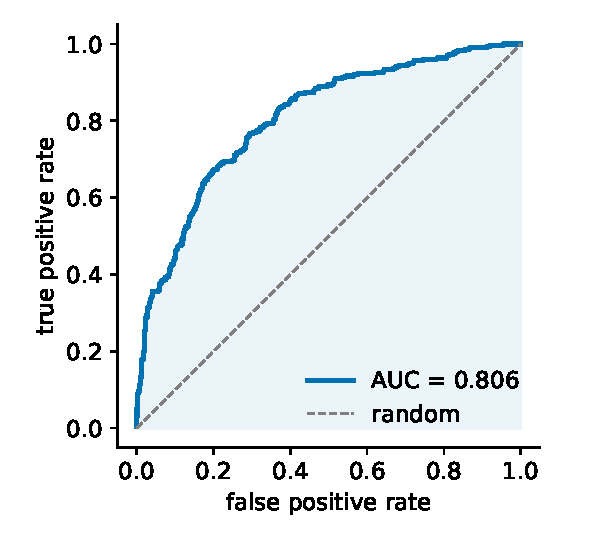
\includegraphics[width=0.9\textwidth]{fig_roc.pdf}
\end{column}
\begin{column}{0.56\textwidth}
\begin{itemize}
  \item $\tau\to\infty$: nothing positive, $(0,0)$. $\tau\to-\infty$: everything positive, $(1,1)$.
  \item A random score gives the diagonal. Perfect separation gives the corner $(0,1)$.
  \item \textbf{AUC} = area under the curve. Threshold-free; invariant to monotone transforms of $s$.
  \item Precision--recall curves and \textbf{average precision} do the same with (recall, precision), and are
        preferable when positives are rare: FPR barely moves when TN is huge.
\end{itemize}
\end{column}
\end{columns}
\end{frame}

\begin{frame}{What AUC Actually Measures}
\begin{claim}{AUC $=\Prob\bigl(s(\vx^+)>s(\vx^-)\bigr)$ for a random positive $\vx^+$ and a random negative $\vx^-$}
\end{claim}
\begin{derivation}{Proof for the empirical curve, $N_+$ positives and $N_-$ negatives, distinct scores}
Sort all scores. Moving $\tau$ down past a \emph{negative} moves the curve right by $1/N_-$; past a
\emph{positive}, up by $1/N_+$. The curve is a staircase, and its area is the sum, over each negative, of the
height of the curve when that negative is crossed:
\[
\text{AUC}=\sum_{\text{neg }j}\frac1{N_-}\cdot\frac{\#\{\text{pos }i:\ s_i>s_j\}}{N_+}
=\frac{1}{N_+N_-}\sum_{i\in+}\sum_{j\in-}\ind{s_i>s_j}.\qquad\qed
\]
\end{derivation}
\begin{itemize}
  \item This is the Mann--Whitney $U$ statistic. AUC is a rank statistic, which is why it ignores calibration.
  \item An AUC of $0.5$ means the scores carry no ranking information. Below $0.5$ means flip the sign.
\end{itemize}
\end{frame}

\begin{frame}{Costs Are Asymmetric: Choosing the Threshold}\footnotesize
Suppose a false positive costs $c_{\text{FP}}$ and a false negative costs $c_{\text{FN}}$, and the classifier
outputs a calibrated $p(\vx)=\Prob(y=1\mid\vx)$.
\begin{derivation}{Minimize expected cost at $\vx$}
\begin{align*}
\text{Predict }1:&\quad\E[\text{cost}]=(1-p)\,c_{\text{FP}} && \text{(wrong iff }y=0\text{)}\\
\text{Predict }0:&\quad\E[\text{cost}]=p\,c_{\text{FN}} && \text{(wrong iff }y=1\text{)}
\end{align*}
Predict $1$ iff $(1-p)c_{\text{FP}}\le p\,c_{\text{FN}}$, i.e.
\[
\boxed{\ \hat y=1\iff p(\vx)\ \ge\ \tau^\star=\frac{c_{\text{FP}}}{c_{\text{FP}}+c_{\text{FN}}}\ }
\]
\end{derivation}
\begin{itemize}
  \item Equal costs: $\tau^\star=\tfrac12$ --- the Bayes classifier.
  \item A false negative ten times worse than a false positive: $\tau^\star=1/11\approx0.09$. Predict positive
        on weak evidence, because missing one is expensive.
  \item The threshold is a property of the \emph{decision}, not of the model. Train for probabilities (log loss),
        then choose $\tau$ from the costs. Never bake the costs into the training labels.
\end{itemize}
\end{frame}

\begin{frame}{Multiclass, Briefly}
For $K>2$ classes the confusion matrix is $K\times K$, and each class $k$ has its own precision and recall
(one-vs-rest).
\begin{itemize}
  \item \textbf{Macro} average: mean of the per-class scores. Every class counts equally, however rare.
  \item \textbf{Micro} average: pool all TP, FP, FN, then compute once. Equals accuracy for single-label problems.
  \item Report the full matrix when $K$ is small. Most errors have structure --- two classes confused with each
        other --- that no average shows.
\end{itemize}
\vspace{6pt}
\begin{keypoint}
The metric is part of the problem statement, not of the method. Decide it before fitting anything.
\end{keypoint}
\end{frame}

% =============================================================================
\sectionframe{Summary}
% =============================================================================

\begin{frame}{What We Proved Today}
\begin{enumerate}
  \item Ridge: $\hat\vbeta_\lambda=(\vX\T\vX+\lambda\vI)\inv\vX\T\vy$, unique for all $\lambda>0$; in the SVD basis it
        shrinks direction $j$ by $d_j^2/(d_j^2+\lambda)$; $\mathrm{df}(\lambda)=\sum_jd_j^2/(d_j^2+\lambda)$; it is the
        posterior mode under a Gaussian prior with $\lambda=\sigma^2/\tau^2$.
  \item Penalized and constrained formulations are equivalent (one direction elementary, the other via Slater).
  \item Lasso with orthonormal $\vX$: $\hat\beta_j=\sign(b_j)(\abs{b_j}-\lambda)_+$. In general, $\hat\beta_j=0$ iff
        $\abs{\vx^{(j)\top}\vr}\le\lambda$; coordinate descent applies soft thresholding one coordinate at a time.
  \item Optimism of training error $=2\sigma^2\,\mathrm{df}/N$.
  \item AUC $=\Prob(s^+>s^-)$; the cost-optimal threshold is $c_{\text{FP}}/(c_{\text{FP}}+c_{\text{FN}})$.
\end{enumerate}
\end{frame}

\begin{frame}{Next}
\textbf{Lab 2 (Wednesday, Rodrigo)} --- ridge and lasso paths on real data, cross-validated $\lambda$ with the
one-SE rule, and what regularization does to logistic regression on separable data.
\vspace{8pt}

\textbf{Lecture 4 (Friday)} --- a different hypothesis class altogether: decision trees. Impurity measures
and why concavity matters, information gain, greedy training, and bagging --- the first method that reduces
variance without touching bias.
\vspace{8pt}

\textbf{Reading} --- \emph{ESL} \S3.4 (ridge, lasso), \S3.8.6 (coordinate descent), \S7.4--7.5 (optimism, $C_p$),
\S7.10 (cross-validation). Tibshirani (1996) for the lasso in the original.
\end{frame}

\end{document}
